\documentclass[a4paper]{article}
\usepackage[utf8]{inputenc}
\usepackage[german]{babel}
\usepackage{underscore}
\usepackage{xcolor}
\usepackage{listings}
\usepackage{graphicx}
\usepackage{hyperref}

\usepackage{xparse}

\NewDocumentCommand{\codeword}{v}{%
\texttt{\textcolor{blue}{#1}}%
}

\lstset{language=VHDL,keywordstyle={\bfseries \color{purple}}}

\title{ERA-Projekt 2 - Dokumentation}
\author{Korbinian Stein}
\begin{document}
    \maketitle
    \tableofcontents
    \section{Allgemeine Programmbeschreibung}
        \subsection{Hauptprogramm} \label{hauptprogramm}
            Der entwickelte Baustein ist ein Konverter, 
            der parallele Signale annimmt und diese seriell wieder ausgibt.
            Im Folgenden werden die Form der erwarteten Eingaben, sowie die daraus 
            resultierenden Ausgaben definiert.
            Die Eingaben sollten an folgenden Ports anliegen:\\

            \noindent \begin{tabular}{l | c | c }
                Port-Name & Typ & Erwartete Daten \\
                \hline
                \codeword{clk} & \codeword{std_logic} & Takt-Signal (Der Baustein reagiert auf \codeword{rising_edge}) \\
                \codeword{S} & \codeword{std_logic} & Gibt an ob der Speicher gesperrt ist (\codeword{HIGH} $\Rightarrow$ gesperrt)\\
                \codeword{input} & \codeword{std_logic_vector} & Adressensignal auf 16 Leitungen \\
            \end{tabular}
            \\

            \noindent Das Signal \codeword{S} unterbricht eine laufende serielle Ausgabe nicht, 
            es wird lediglich benutzt um den Start einer Konvertierung zu verzögern, 
            bis neue zu konvertierende parallele Daten auf \codeword{input} bereitliegen.
            Das parallele \codeword{input}-Signal sollte aus der Strangsteuerung von Leitung 0-7 
            und aus der Lampensteuerung von Leitung 8-15 bestehen.
            
            Die Ausgabe erfolgt auf folgenden Ports:\\

            \noindent \begin{tabular}{l | c | c}
                Port-Name & Typ & Ausgegebene Daten\\
                \hline
                \codeword{out0} & \codeword{std_logic} & Serielle Ausgabe für Strangsteuerung (\codeword{input} 0-7)\\
                \codeword{out1} & \codeword{std_logic} & Serielle Ausgabe für Lampensteuerung (\codeword{input} 8-15)\\
            \end{tabular}
            \\

            \noindent Die Ausgabe erfolgt stückweise jedes \codeword{rising_edge} und dauert insgesamt 32 Takte. 
            Der Beginn der Ausgabe ist aus technischen Gründen jeweils um einen Takt nach hinten verschoben; Daraus resultierend beginnen die 32 Takte ab dem zweiten Takt, nachdem das \codeword{S}-Signal nicht anlag.
             Das Protokoll für die Ausgabe ist genau definiert:

            \begin{tabular}{c | c}\label{protokoll}
                Takt-Zahl  & Verhaltensweise \\
                \hline
                $1-4$   & Start-Ausgabe an Strangsteuerung \\
                $5-12$  & Daten-Ausgabe an Strangsteuerung\\
                $13-16$ & Stop-Ausgabe an Strangsteuerung\\
                \hline
                $17-20$   & Start-Ausgabe an Lampensteuerung\\
                $21-28$  & Daten-Ausgabe an Lampensteuerung\\
                $29-32$ & Stop-Ausgabe an Lampensteuerung\\
              \end{tabular}\\

              Das hier erwähnte Start-Signal besteht aus einem Takt \codeword{HIGH} und zwei Takten \codeword{LOW}, 
              danach beginnt die Daten-Ausgabe. 
              Das Stop-Signal besteht aus einem Takt \codeword{LOW} und zwei Takten \codeword{HIGH}.
        \subsection{Tests}
            Für den Test des Bausteins wurde eine der \codeword{GHDL}-Spezifikation entsprechenden \codeword{Testbench} erstellt.
            Diese legt mithilfe von \codeword{GHDL} virtuell definierte Signale an den Baustein an und vergleicht dessen Ausgänge mit dem erwarteten Verhalten.
            Zusätzlich wird eine Datei mit den Daten in Wellenform erstellt, 
            welche sich z.B. mit GTKWave öffnen lässt, um eine graphische Repräsentation der Ein- und Ausgaben betrachten zu können.
   
\section{Nutzerdokumentation}
   \subsection{Verwendung} \label{Verwendung}
   			Zur Ausführung der Tests und Benutzung des Bausteins in anderen Projekte werden weitere Programme benötigt. Diese organisieren den Prozess des Kompilierens und werden zur verbesserten Nachvollziehbarkeit, insbesondere von Tests, genutzt.
   			Wichtig sind:\\
   			
   			\begin{tabular}{c | c | p{60mm}}
   				Programm & Getestete Version & Funktionalität\\
   				\hline
   				ghdl & 0.29 & Erzeugt aus VHDL-Quelltext ausführbare Dateien\\
   				make & 4.1 & Liest die Definition des Kompilier-Prozesses und führt diesen entsprechend aus, um einen einheitlichen Ablauf zu gewährleisten\\
   				gtkwave & 3.3.66 & Stellt die von \codeword{ghdl} erzeugten Wellenformen in einem Diagramm dar, damit diese nachvollziehbarer werden\\
   			\end{tabular}
   			\\
   			
   			\noindent Alle Tests wurden auf \codeword{Ubuntu 16.04 32-Bit} durchgeführt. Andere Versionen des Betriebssystem oder der benötigten Programme sollten ebenso funktionieren, da keine besonderen, versionsspezifischen Features genutzt werden. Allerdings kann der reibungsfreie Ablauf mit einer anderen Konfiguration nicht garantiert werden.
   			
   				
   		\subsection{Kompilieren und Ausführen}
   			Nach dem Klonen des Projektes befinden sich im Ordner \emph{Implementation} lediglich die benötigten Quelldateien. Diese müssen mit \emph{ghdl} kompiliert werden, um ein ausführbares Programm zu erzeugen. Hierzu kann das mitgelieferte \codeword{makefile} genutzt werden. Ruft man also aus dem Ordner \codeword{make} auf, so überprüft dieses alle notwendigen Abhängigkeiten und erzeugt die benötigten ausführbaren Dateien (siehe Abb. \ref{fig:screenshot001}).
   			
   			\begin{figure}[hb]
   				\centering
   				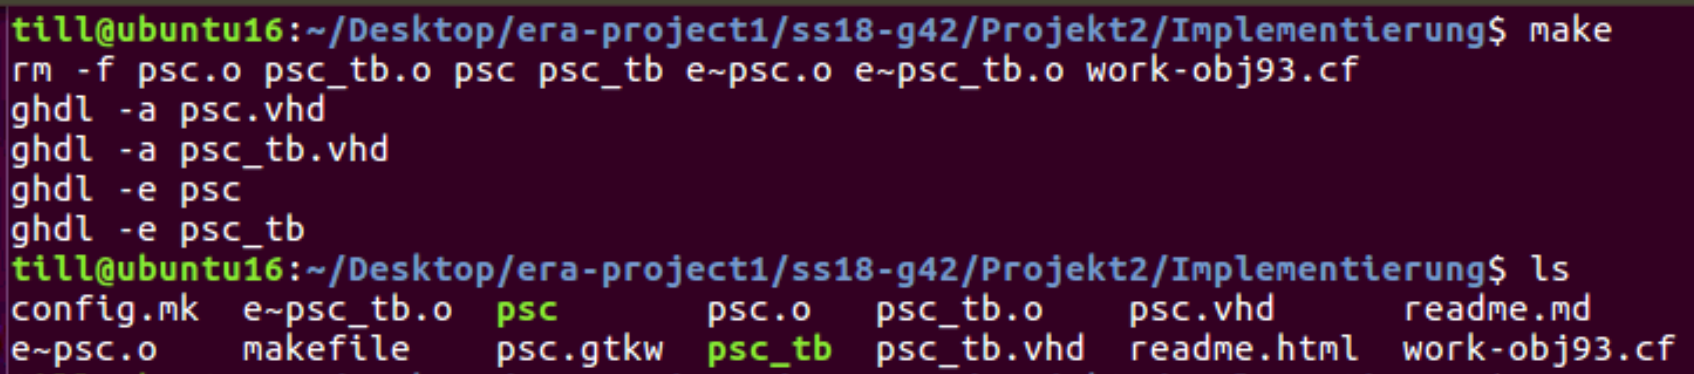
\includegraphics[width=0.7\linewidth]{images/screenshot001}
   				\caption{Ausgabe von \emph{make} und Inhalt des Ordners nach dem Kompilieren}
   				\label{fig:screenshot001}
   			\end{figure}
   			
   			Daraufhin kann das Programm mit \codeword{make run} ausgeführt werden. Es läuft nun die Simulation für 32 Takte durch und die dabei aufgezeichnete Wellenform wird in der Datei \emph{psc_tb.ghw} gespeichert. Nach erfolgreichem Abschluss der Simulation wird die Wellenform in \emph{gtkwave} geöffnet und alle wichtigen Felder automatisch angezeigt (siehe Abb. \ref{fig:screenshot004}).
   			
   			\begin{figure}[hb]
   				\centering
   				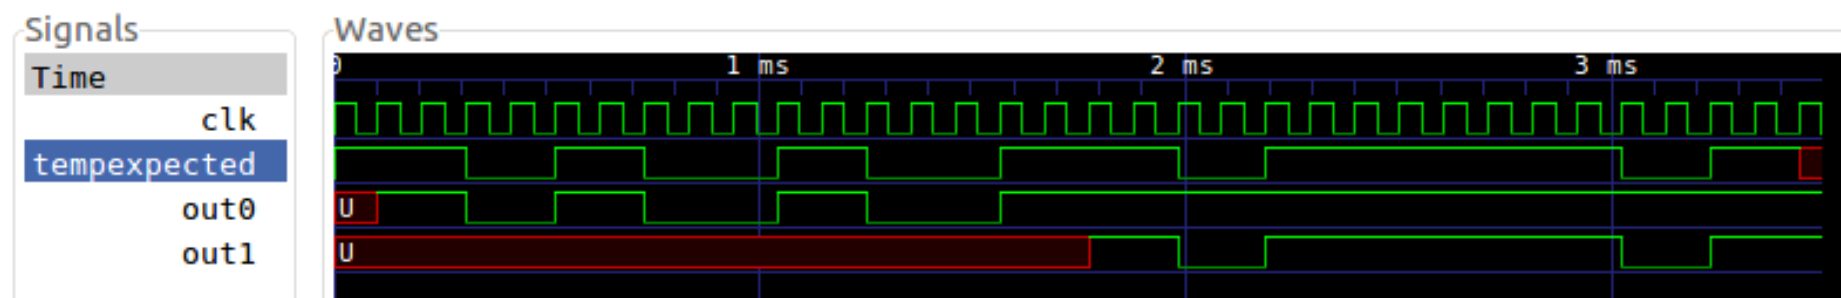
\includegraphics[width=0.7\linewidth]{images/screenshot004}
   				\caption{\emph{gtkwave} nach der erfolgreichen Simulation. Für die ersten 16 Takte entspricht \emph{tempexpected out0}, für die weiteren Takte entspricht es \emph{out1}}
   				\label{fig:screenshot004}
   			\end{figure}
   		
   		\newpage
   		Allgemein bietet das Makefile folgende Befehle: \\ \\
	   		\begin{tabular}{c | l } \label{make-befehle}
	   			Befehl & Aktion\\
	   			\hline
	   			\codeword{make} & Kompiliert das Projekt\\
	   			\codeword{make run} & Führt Tests aus und zeigt das Ergebnis in \emph{gtkwave}\\
	   			\codeword{make clean} & Löscht alle durch \codeword{make run} erzeugten Dateien\\
	   		\end{tabular}
	   	
   			
   	\subsection{Tests} \label{tests}
   		\subsubsection{Andere Tests ausführen}
   			Standardmäßig führt das Programm den ersten mitgelieferten Test aus. Dieser enthält zufällige Zahlen und überprüft damit, dass Signale vom Baustein nicht verändert werden, sowie dass das Protokoll richtig umgesetzt wird.
   			
			   In der Datei \codeword{psc_tb.vhd} sind noch zwei weitere Tests enthalten. Der zweite Test ähnelt dem ersten, nutzt jedoch andere Zahlen. Der dritte Test 
			   hingegen überprüft das Verhalten des Programms bei unerwarteten Eingaben, indem er undefinierte Zustände übergibt. Auch diese sollten vom Baustein problemlos verarbeitet und wieder ausgegeben werden.\\
   			
			   \noindent Nach einer Änderung der Tests muss \codeword{make} erneut aufgerufen werden,
			    um die Binärdateien mit den neuen Daten zu erstellen. Danach wird der Test wie gewohnt mit \codeword{make run} gestartet.
   			
   		\subsubsection{Testergebnisse auswerten}

			   Grundsätzlich gibt es zwei Möglichkeiten den Erfolg eines Tests zu bestimmen. Zunächst überprüft die Testbench schon während der Simulation, 
			   ob die erwarteten Werte den tatsächlichen Werten entsprechen. Ist dies nicht der Fall, so wird in der Konsole eine Meldung ausgegeben, 
			   die darauf hinweist. Zusätzlich wird der erwartete und tatsächliche Wert zusammen mit der aktuellen Position der Zählvariable aus (siehe Abb. \ref{fig:screenshot002})
   			
   			\begin{figure}[hb]
   				\centering
   				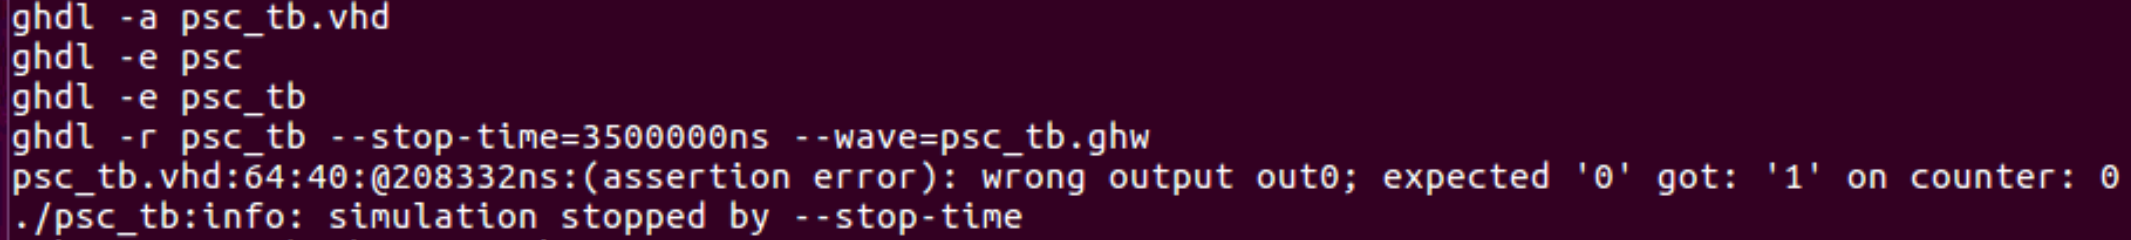
\includegraphics[width=0.7\linewidth]{images/screenshot002}
   				\caption{Ausgabe von \emph{make run} mit Fehlermeldung in Zeile 5}
   				\label{fig:screenshot002}
   			\end{figure}
   			
			   Zur weiteren Analyse eines Problems, wird nach dem Ende der Simulation \emph{gtkwave} gestartet. 
			   Interessant sind vor allem die Signale \codeword{temp_expected}, \codeword{out0} und \codeword{out1}, welche sich wie in Abb. \ref{fig:screenshot004} 
			   beschrieben zueinander verhalten sollten. Fehlermeldungen der Testbench lassen sich mit \emph{gtkwave} weiter untersuchen (siehe Abb. \ref{fig:screenshot003})
   			
   			\begin{figure}[hb]
   				\centering
   				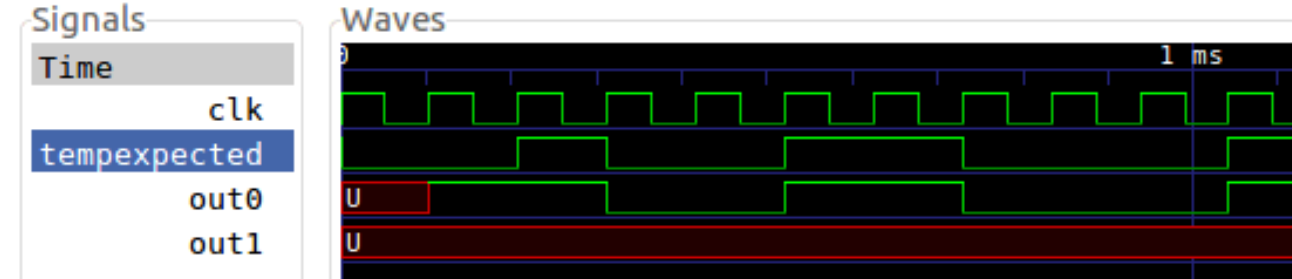
\includegraphics[width=0.7\linewidth]{images/screenshot003}
   				\caption{\emph{gtkwave} nach fehlgeschlagenem Test - \emph{tempexpected} stimmt im zweiten Takt nicht mit \emph{out0} überein}
   				\label{fig:screenshot003}
   			\end{figure}
   			
   		\subsubsection{Eigene Tests definieren}
			   Möchte man nun eigene Tests definieren, so ist dies am einfachsten möglich, indem man zwei eigene \codeword{std_logic_vector} anstelle der durch die Tests gegebenen definiert. 
			   Hierzu sind Änderungen an zwei Stellen im Code der \codeword{psc_tb.vhd} notwendig:
   			\begin{enumerate}
				   \item In Zeile 27 - 29 einen der Tests kopieren oder verändern, sodass der \mbox{\emph{std_logic_vector expected}} die erwartete Ausgabe enthält. 
				   Dabei wird während des Tests die rechte Hälfte von \emph{expected} mit \emph{out0} verglichen, die linke Hälfte mit \emph{out1}.
				   \item In Zeile 42 - 44 die Eingabewerte an die gerade erstellten Erwartungswerte anpassen. 
				   Hierfür kann auch entweder eine bestehende Zeile bearbeitet oder eine neue erstellt werden, \emph{std_logic_vector input} muss die passenden Eingabewerte enthalten.
   			\end{enumerate}
   		
   			\noindent Nun kann identisch zu den vorgegebenen Tests \codeword{make} und danach \codeword{make run} aufgerufen werden, um den neuen Test zu starten.
   			
   		\subsection{Verwendung als Teil eines Systems}
		   Der Baustein lässt sich problemlos als Teil eines größeren Systems benutzen. Hierbei ist vor allem die Belegung der Ein- und Ausgänge wie in Abschnitt \ref{hauptprogramm} beschrieben zu beachten.
		    Solange die alle Daten entsprechend am Baustein ankommen, kann mit den Tests aus Abschnitt \ref{tests} die korrekte Funktionalität gewährleistet werden.
            
    \section{Entwicklerdokumentation}
		\subsection{Allgemeine Informationen}
			Das implementierte System besteht aus zwei Quellcode-Dateien, dem Baustein \codeword{psc.vhd} und der Testbench \codeword{psc_tb.vhd}. 
			Alle weiteren Dateien enthalten Informationen für den Anwender, Konfigurationen für das Kompilieren und Anzeigen der Wellen-Dateien. Diese werden im Abschnitt \ref{KompilierProzess} genauer behandelt.\\
			Ohne ein System, in dem der Baustein integriert wird, können lediglich Tests auf dem Baustein ausgeführt werden. 
			Alle hierfür benötigten Abhängigkeiten werden im Abschnitt \ref{Verwendung} beschrieben.
        \subsection{psc.vhd}
        \subsubsection{Konzept}
        	Der Baustein implementiert das in Abschnitt \ref{hauptprogramm} definierte Protokoll. Folgende Schritte werden dafür nacheinander ausgeführt:\\
        	\begin{enumerate}
        		\item Die interne Zählvariable \codeword{counter} auf \codeword{0} setzen
        		\item Falls das Sperrsignal \codeword{S} anliegt, warten, bis es nicht mehr anliegt
        		\item Den Eingang \codeword{input} in das interne Signal \codeword{data} lesen. Dies macht das Programm nach dem Einlesen unabhängig davon, ob die Eingänge über den kompletten Zeitraum der Ausgabe anliegen, oder nicht.
        		\item Jeden Takt die Zählvariable um \codeword{1} erhöhen und dabei die entsprechenden Protokoll- oder Datenbits an den richtigen Ausgang schreiben. Dieser Vorgang entspricht einer \emph{State-Machine} (siehe Abb. \ref{fig:statemachine}).
        		\item Sobald die Zählvariable \codeword{32} erreicht, wird sie wieder auf \codeword{0} zurückgesetzt und ist damit bereit, die nächsten Eingabedaten zu verarbeiten.
        	\end{enumerate}
			\emph{Anmerkung} \label{sperrsignal-anmerkung}: Wird das Sperr-Signal \codeword{S} während der Ausgabe aktiviert, so wird diese nicht unterbrochen, sondern läuft durch, 
			um zu gewährleisten, dass ausschließlich vollständige Daten an die weiteren Bausteine gegeben werden. 
			Sobald die Ausgabe erfolgt ist, wartet der Baustein auf die Aufhebung der Sperre, bevor er mit dem nächsten Datensatz fortfährt.\\
        	
        	\noindent Der Baustein enthält keinen eigenen Taktgeber, stattdessen muss diese über den Eingang \codeword{clk} extern angelegt werden.
        
           	\begin{figure}[hb]
        		\centering
        		\includegraphics[width=1.2\linewidth]{images/Statemachine}
        		\caption{Zustandsdiagramm der Umsetzung des Protokolls \newline \emph{Anmerkung: Das Diagramm ist aus der Spezifikation übernommen!}}
        		\label{fig:statemachine}
        	\end{figure}
        
        \subsubsection{Umsetzung}
        	Die Umsetzung des Konzeptes ist relativ direkt. Zunächst werden die Ports wie in Abschnitt \ref{hauptprogramm} beschrieben definiert und im Anschluss die internen Signale wie folgt:\\
        	
        	\begin{tabular}{c | c | l}
        		Name & Typ & Funktion\\
        		\hline
        		\codeword{counter} & \codeword{unsigned(5 downto 0)} & Zählvariable für die \emph{State-Machine}\\
        		\codeword{data} & \codeword{std_logic_vector(15 downto 0)} & Interne Duplizierung der Eingabedaten\\
        		\codeword{out0_intern} & \codeword{std_logic} & Interne Duplizierung von \codeword{out0}\\
        		\codeword{out1_intern} & \codeword{std_logic} & Interne Duplizierung von \codeword{out1}\\
        	\end{tabular}\\ \\
		\emph{Anmerkung}: \codeword{out0_intern} und \codeword{out1_intern} werden per \codeword{concurrent-statement} auf die externen Ports \codeword{out0} und \codeword{out1} gelegt. 
		Dies erlaubt mehr Flexibilität beim Entwickeln des Bausteins, da von den beiden internen Signalen direkt gelesen werden kann.\\ \\
		Der Baustein selbst besteht aus einem Prozess, der ausschließlich auf \codeword{rising_edge(clk)} reagiert 
		und das Zustandsdiagramm per \codeword{if [...] elsif [...] ...} umsetzt. Wie in Abbildung \ref{fig:statemachine} gezeigt, 
		wird in den ersten vier Takten das Startsignal des Protokolls (siehe \ref{protokoll}), gefolgt von den ersten acht Datenbits und dem Endsignal des Protokolls auf \codeword{out0} ausgegeben.
		Anschließend findet die gleiche Ausgabe, jedoch mit der zweiten Hälfte der Daten, auf \codeword{out1} statt. 
		Für die Ausgaben werden die Signale \codeword{out0_intern} und \codeword{out1_intern} entsprechend der gewünschten Ausgabe belegt.\\ \\
		Wichtig ist dabei, dass die richtigen Daten aus \codeword{data} passend zur Zählvariable genutzt werden. 
		Da die Zählvariable aber natürlich auch andere Zustände, vor allem die Ausgabe der Protokollbits, umfasst, 
		ist bei \codeword{out0_intern} eine Verschiebung von \codeword{counter} um \codeword{-4} notwendig.
        
        Durch die acht benötigten Protokollausgaben zwischen dem ersten und dem zweiten Teil der Ausgabe, erhöht sich für \codeword{out1_intern} die Verschiebung auf \codeword{-12}.\\ \\
		Nachdem nun das richtige Bit für den aktuellen Zustand ausgegeben wurde, wird die Zählvariable entsprechend der Beschreibung (siehe \ref{sperrsignal-anmerkung}) verändert.
		Sollte sie dabei \codeword{32} erreichen, wird ihr der Wert \codeword{0} zugewiesen; Der Baustein ist bereit für die nächsten Eingabedaten.
        		
        
        \subsection{psc_tb.vhd}
        
        	\subsubsection{Konzept}
				Die Testbench implementiert eine Testumgebung für \codeword{psc.vhd} und nutzt dafür eine einfache Vergleichslogik, 
				die Differenzen zwischen dem tatsächlichen und dem erwarteten Ergebnis erkennt und meldet. Die Vorgehensweise ist dabei wie folgt:\\
        		\begin{enumerate}
        			\item Den Baustein initialisieren und seine Ein- und Ausgänge auf interne Signale legen (insbesondere die Clock)
        			\item Den vorgegebenen \codeword{input} an den Baustein ausgeben
        			\item Für einen Takt warten, bis der Baustein bereit ist
        			\item Die Zählvariable jeden Takt um \codeword{1} erhöhen und bei \codeword{counter < 16} den entsprechenden, erwarteten Wert mit \codeword{out0} vergleichen
        			\item Ist \codeword{counter} größer oder gleich \codeword{16}, den erwarteten Wert mit \codeword{out1} vergleichen
        			\item Ist \codeword{counter = 32}, so wird er wieder auf \codeword{0} gesetzt
        		\end{enumerate}
			\emph{Anmerkung} \label{stop-time-anmerkung}: Da die Clock eine festgelegte Geschwindigkeit von 9600 Takten pro Sekunde hat, 
			kann bei Ausführen der Testbench mithilfe des Arguments \codeword{--stop-time} die Simulation nach der gewünschten Anzahl von Durchläufen gestoppt werden.
        	
        	\subsubsection{Umsetzung}
        	
			 Die Ports der Testbench entsprechen denen des zu testenden Bausteins, jedoch gibt es einige interne Signale, um Eingaben bereitzustellen und Ausgaben zu verarbeiten.
			 Zunächst gibt es für jeden Ein- und Ausgang des Bausteins ein internes Signal, welches dann jeweils auf den entsprechenden Port des Bausteins gelegt wird:\\ \\
        	\begin{tabular}{c | c}
        		Name & Typ\\
        		\hline
        		\codeword{clk} & \codeword{std_logic}\\
        		\codeword{S} & \codeword{std_logic}\\
        		\codeword{out0} & \codeword{std_logic}\\
        		\codeword{out1} & \codeword{std_logic}\\
        		\codeword{input} & \codeword{std_logic_vector}\\
        	\end{tabular}\\ \\
        	Die Testbench besitzt jedoch noch einige weitere Signale um den Baustein testen zu können:\\ \\
        	\begin{tabular}{c | c | l}
        		Name & Typ & Funktion\\
        		\hline
        		\codeword{expected} & \codeword{std_logic_vector} & Enthält den erwarteten Datenstrom.\\
        		&& Die erste Hälfte des Signales wird dabei beim\\
        		&& Testen mit \codeword{out0} verglichen,\\
        		&& die zweite Hälfte mit \codeword{out1}\\
        		\codeword{tempExpected} & \codeword{std_logic} & Enthält das nächste erwartete Bit\\
        		\codeword{waitOnce} & \codeword{std_logic} & Wird einmalig beim Start der Testbench\\
        		&& genutzt, um Baustein und Testbench zu\\
        		&& synchronisieren, da der Baustein erst einen\\
        		&& Takt später verfügbar ist.\\
        		\codeword{done} & \codeword{std_logic} & Wurde benutzt, um die Testbench zu beenden,\\
        		&& sobald der Test durchgelaufen ist. Diese\\
        		&& Funktionalität wird nun durch \codeword{--stop-time}\\
        		&& beim Ausführen der Testbench bereitgestellt\\
        		&& (siehe \ref{stop-time-anmerkung}).\\
        		\codeword{counter} & \codeword{unsigned(5 downto 0)} & Zählvariable, damit der erwartete Wert mit\\
        		&& dem richtigten Ausgang verglichen werden\\
        		&& kann.\\
        	\end{tabular}
        		
        \begin{figure}[hb]
        	\centering
        	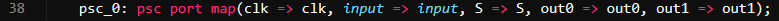
\includegraphics[width=1.2\linewidth]{images/screenshot005}
        	\caption{\emph{psc_tb.vhd, Zeile 38} - Zuweisung der internen Signale auf die Ports des Bausteins}
        	\label{fig:screenshot005}
        \end{figure}
    
		\noindent Zunächst werden die Ports des Bausteins den entsprechenden internen Signalen zugeordnet (siehe Abb. \ref{fig:screenshot005}). Daraufhin legt die Testbench \codeword{input} an den Baustein an 
		und setzt \codeword{tempExpected} auf den jeweils nächsten, von der Zählvariable abhängigen, Erwartungswert.\\ \\
		Wie auch der Baustein enthält die Testbench einen Prozess, der auf die Clock reagiert. 
		Nach einmaligem Warten beim Start der Ausführung wird lediglich die Zählvariable nach oben gezählt und über einen \codeword{assert} die aktuelle Ausgabe überprüft. 
		Entspricht diese dabei nicht dem Erwartungswert, so wird während der Simulation eine Fehlermeldung (siehe Abb. \ref{fig:screenshot002}) ausgegeben. 
		Da beim Weiterentwickeln oder Ändern des Bausteins nicht nur die falschen, sondern alle Werte interessant sein können, 
		ist über einen gegenteiligen \codeword{assert} auch die Möglichkeit gegeben, alle erhaltenen Bits ausgeben zu lassen. 
		Da diese Daten für den Anwender jedoch meist uninteressant sind, sind die entsprechenden Befehle auskommentiert.
        
		Erreicht die Zählvariable einen Wert von \codeword{32}, so wird sie wieder auf \codeword{0} gesetzt und der Test läuft von vorne durch. 
		Dies passiert dabei synchron mit dem Baustein, ein weiterer Warte-Takt mithilfe von \codeword{waitOnce} ist somit also nicht nötig.
        
        \subsection{Build-Prozess} \label{KompilierProzess}
        	\subsubsection{make}
				Zum einfachen und einheitlichen Kompilieren des Projektes existiert ein \codeword{makefile}, welches zusammen mit \codeword{config.mk} eine Konfiguration für \codeword{make} bereitstellt. 
				Die Befehle können dabei aus Abschnitt \ref{make-befehle} entnommen werden. 
				Zum Kompilieren und Ausführen von Baustein und Testbench wird \codeword{ghdl} benutzt, ebenso zum Simulieren für Tests. Die dabei erstellte Wellenform wird in der Datei \codeword{psc_tb.ghw} abgespeichert.
        	\subsubsection{gtkwave}
				\codeword{make run} öffnet nach dem Durchlauf der Simulation \emph{gtkwave} mit der erstellen Wellenform-Datei, sowie der Konfigurationsdatei \codeword{psc.gtkw}.
				 Diese sorgt dafür, dass \emph{gtkwave} sofort alle relevanten Daten anzeigt und die GUI nicht erst noch vom Anwender eingestellt werden muss.
        	\subsubsection{readme}
				Zur schnellen Übersicht für Benutzer und Entwickler enthält das Projekt zusätzlich noch eine Readme-Datei, 
				die die wichtigste Eigenschaften und Befehle des Bausteins und der Testbench zusammenfasst. 
				Die Datei ist als Markdown-Version in \codeword{readme.md}, sowie als HTML-Version in \codeword{readme.html} gespeichert.
         
\end{document}
